\documentclass[a4paper,10pt]{article}
\usepackage[utf8]{inputenc}
\usepackage[backend=bibtex]{biblatex}
\usepackage{filecontents}
\usepackage{graphics}
\usepackage[usenames,dvipsnames]{xcolor}
\usepackage{amsmath,amssymb,amsfonts,mathrsfs}
\usepackage{cancel}
\usepackage{mathtools}
\usepackage{ifthen}
\usepackage{minibox}
\usepackage{color}
\usepackage{bigdelim, bigstrut}
\usepackage{tocloft}
\usepackage{framed}
\usepackage{enumitem}

\usepackage[left=20mm,right=20mm,top=20mm,bottom=20mm,foot=10mm]{geometry}


%%%%%%%%%%%%%%%%%%%%%%%%%%%%%%%%%%%%%%%%%%%%%%%%%%%%%%%%%%%%%%%%%%%%%%%%%%%%%%%%%%%%%
%% CODE LISTINGS for source code of different programming languages in color
\usepackage{listings}
\usepackage{color}
\usepackage{textcomp}
\lstdefinelanguage{JavaScript}{
  keywords={typeof, new, true, false, catch, function, return, null, catch, switch, var, if, in, while, do, else, case, break},
  keywordstyle=\color{blue}\bfseries,
  ndkeywords={class, export, boolean, throw, implements, import, this},
  ndkeywordstyle=\color{darkgray}\bfseries,
  identifierstyle=\color{black},
  sensitive=false,
  comment=[l]{//},
  morecomment=[s]{/*}{*/},
  commentstyle=\color{purple}\ttfamily,
  stringstyle=\color{red}\ttfamily,
  morestring=[b]',
  morestring=[b]"
}


\definecolor{listinggray}{gray}{0.9}
\definecolor{lbcolor}{rgb}{0.9,0.9,0.9}
\lstset{
	backgroundcolor=\color{lbcolor},
	tabsize=4,
	rulecolor=,
	language=JavaScript,
	numbers=left,
	numberstyle=\footnotesize,
        basicstyle=\scriptsize,
        upquote=true,
        aboveskip={0.3\baselineskip},
        columns=fixed,
        showstringspaces=false,
        extendedchars=true,
        breaklines=true,
        prebreak = \raisebox{0ex}[0ex][0ex]{\ensuremath{\hookleftarrow}},
        frame=single,
        showtabs=false,
        showspaces=false,
        showstringspaces=false,
	basicstyle=\small\ttfamily,
        identifierstyle=\ttfamily,
%         keywordstyle=\color[rgb]{0,0,1},
        commentstyle=\color[rgb]{0.133,0.545,0.133},
        stringstyle=\color[rgb]{0.627,0.126,0.941},
}
%% end code listings
%%%%%%%%%%%%%%%%%%%%%%%%%%%%%%%%%%%%%%%%%%%%%%%%%%%%%%%%%%%%%%%%%%%%%%%%%%%%%%%%%%%%%









%opening
\title{Github Events Data Documentation DRAFT}
\author{Thomas Gersdorf}

\addbibresource{smi.bib}

\setlength\parindent{0cm}


\setcounter{tocdepth}{2}
\input{../../math_setup/thg_math_setup.tex} % include math macros


\begin{document}

\maketitle


\tableofcontents


\section{Fundamental and Derived Measures}
\subsection{Terminology}
\begin{description}
\item [Repository] A repository is the basic 'project' unit in language of software development. A user or an organization can have many software repositories. Each repository typically has branches (very often with a 'main' branch) which represent different development streams within the project. A repository typically also releases ready pieces of software.
\item[Issue] An issue is a generalized form of everything which should be improved on a piece of software, like for instance bug reports or new feature requests.
\item [Commit] A commit is the action of submitting new code to the repository. Typically, commits are made \textbf{decentralized}, which means that the developer is typing "commit" on his own computer. One or several commits can be uploaded via a push.
\item [Push ] A push is a the action of uploading committed source code to the repository. It's one of the key features of Git's decentralized environment. During a push event, editing conflicts can emerge and then need to be resolved.
 \item[Gist] Gists are snippets of code to be shared with others, interdependent of a repository. Can be cloned, forked etc. like a repository, not super important here.
\item [Fork] Forks are clones/copies of a repository or Gist into a User's own account. The can be used to parallelize development of the project, the feedback to the original project can be done via \textit{PullRequests.}
\item [PullRequest] A user submits his additions/changes and asks the owners of the repository to include his changes into the original project ('\textit{pulling}')
\item [Payload] The contents of an action (like the source code itself, the comments itself, all acompanying information but not the meta-data such as timestamps.)
\end{description}

Detailed information on Github's Event API can be found in \url{http://developer.github.com/v3/activity/events/types/} .

\subsection{Users/Actors}
\subsubsection{General Measures for all Events}
\begin{itemize}
 \item Login Name
\item Email
\item Gravatar ID
\item Type (User/Organization)
\item Company (if set)
\item Location (if set)
\item Blog (if set)
\end{itemize}


\subsubsection{Event-Specific Measures}
\begin{center}
 
\begin{tabular}{|p{2.5cm}|p{5cm}|p{6cm}|p{2cm}|}\hline
\textbf{Event type} & \textbf{Description}&  \textbf{Contents}& \textbf{\#  for all users in example dataset} \\\hline
 IssuesEvent  & An issues is opened or closed or reopened.   &  Opened, reopened\& closed Issues, Assignee (via API) &29368\\\hline
CreateEvent    &  A repository, branch or tag is created. & Type of created object (repo, branch, tag), name &  116683\\\hline
PushEvent  & Source code is pushed into repository. &  Size, SHA Hash &  298729\\\hline
GistEvent   &  A Gist (source code fragment) is created or updated.  &  Action (created, updated), URL, Gist ID &  26267\\\hline
Issue
CommentEvent &  Comment on an Issue  &  Issue ID, Comment ID, URL to comment, Comment body (via API)   &   45166\\\hline
Commit
CommentEvent &  Comment on a Commit (inline in source code) &  Commit ID, Comment ID, URL, Comment (via API) &  7827\\\hline
ForkEvent   &  Repository is forked.   & Fork URL, Forkee URL    & 19867\\\hline
WatchEvent  & User is watching a repository for changes &  Action (start, stop) &   65193\\\hline
PullRequestEvent     &  Somebody request the repository to pull his changes into the repository.  & Action (opened, closed, synchronize, reopened), PullRequest ID, Contents (files changed, comments, response to issues, etc.), Assginee (via API) ) &  20818\\\hline
PullRequest
ReviewCommentEvent  & A pull request is reviewed by another user. &  Comment details including body (Comment text itself) &  3726\\\hline
FollowEvent   &  A user follows another user, watching is actions.  & Target (Login)  & 17049\\\hline
GollumEvent  &  Update of Wikipages, such as release notes& Page name (e.g. "Release Notes") , Action (created, edited), URL  &  11781\\\hline
DeleteEvent   & Either a branch or tag is removed.   &  Delete Type (Branch or Tag), Name of Deleted Object&   3785\\\hline
MemberEvent   & Users can be made collaborators, thereby given advanced "write" permissions to the repository.   &  Only additions: member(s) added  &    2764\\\hline
DownloadEvent  & A download is created (not \# of downloads.) \red{deprecated (11/2012)! now "release Events".}  &  URL & 2576\\\hline
PublicEvent & A repository is made open-source. &  Repository-URL  &  553\\\hline
TotalEvents & Counts all of the above. & - & 672152 \\\hline
\end{tabular}
\end{center}

\textbf{Non-public events:} TeamAddEvent, StatusEvent (commits), ReleaseEvent (not yet), 

\subsubsection{Constructed Measures for Users}
\begin{description}
 \item [Issues\_Opened] \# of issues the user has opened
 \item [Issues\_Closed] \# of issues the user has closed
\item [Event\_Continuity] $\to$ TODO
\item [Events\_Own] Events on user's repository
\item [Events\_Active\_Involvement] Measure how much the user engages in projects of other user or organizations, events on other repositories 
\item [Events\_Passive\_Involvment] Measures how much other users engage in projects of the user, events on the user's repository by other users
\end{description}



\subsection{Repositories}
\subsubsection{General Measures}
\begin{itemize}
 \item URL (serves as identifier for repos)
\item Name
\item Has downloads? 
\item Has issues?
\item Has wiki?
\item Creation Date
\item Description
\item Number of Forks
\item Repository is fork?
\item Language
\item Private yes/no (only have public data)
\item Owner
\item Parent organization
\item Open Issues
\item Watchers
\item Last Push
\end{itemize}



% {"homepage":"","has_downloads":true,"has_issues":true,"forks":1,"fork":false,"has_wiki":true,"url":"https://github.com/ecloud/90ec2","created_at":"2012/04/10 17:19:08 -0700","size":92,"private":false,"name":"90ec2","description":"","owner":"ecloud","open_issues":0,"watchers":1,"pushed_at":"2012/04/10 17:47:48 -0700"}



\subsubsection{Constructed Measures for Repositories}
\begin{description}
 \item [Distinct\_Contributing\_Users] Number of different users contributing via IssuesEvent, CreateEvent, PushEvent, PullRequestEvent
\end{description}


\section{Constructed Leadership Measures}
\subsection{User: Envisioning and Goal Orientation}

\begin{align}
 LS_{\text{milestone}} = \frac{\text{\# issue directly assigned to a milestone or release}}{\text{\# total issues opened}} 
\end{align}

\textbf{Reasoning:}
Only the core developers know about the schedules for the project and are by social practices allowed to tag issues directly to milestones and releases.




\subsection{User: Leading People}
\subsubsection{Open Issue and Assign  User/Milestone}

\textbf{Measure:}
\begin{align}
 LS_{\text{assign}} = \frac{\text{\# issue directly assigned to other person}}{\text{\# total issues opened}} 
\end{align}


\textbf{Reasoning:}
The more people directly assign users to issues, the more they know about the people's capabilities and empower other users to solve this issue.



\textbf{Control for:}
\begin{itemize}
 \item Total number of issues
\item Size of project
\end{itemize}



Assignee currently only via API from \texttt{ https://api.github.com/repos/thgersdorf/github-play/issues/1
}, see reference.


\subsubsection{User: Taking part in discussions}
\textbf{Measures:}
\begin{align}
 LS_{\text{comments}} = c_{0}\frac{\text{\# issue commented (not own)}}{\text{\# total issues of repo}} +c_{1}\frac{\text{\# PullRequests commented (not own)}}{\text{\# total PullRequests of repo}} 
\end{align}

\textbf{Reasoning:} When a user is is actively commenting on a large fraction of issues or pullrequests, he cares about resolving issues and incorporating improvements. Even though not central LS attribute, important activity measure.




\subsection{User: Empowering}
\textbf{Measure:}

\begin{align}
 LS_{\text{empowerment}} = \frac{\text{\# Comments mentioning somebody else}}{\text{\# All user's comments}}
\end{align}

\textbf{Reasoning:} Measuring how much a users refers to other users in comments, interacts with them (e.g. saying "thanks", "great",...)
TODO: Comments really all measuring empowering leadership?

\textbf{Control:} 
\begin{itemize}
 \item Number of comments
\item Number of different issues for comments
\item Number of different projects for comments
\end{itemize}





\subsection{User: Project Governance}
\subsubsection{Including people in project}

\textbf{Measure:}
\begin{align}
 LS_{\text{governance}} = \frac{\text{\# members added}}{\text{\# members in project}}
\end{align}

\textbf{Reasoning:}

\textbf{Control for:}
\begin{itemize}
 \item Project size
\end{itemize}


\subsubsection{Closing issues | Gatekeepers}
\textbf{Measure:}
\begin{align}
 LS_{\text{governance}} = c_{0}\frac{\text{\# closed issues without commit}}{\text{\# total issues of repo}} + c_{1} \frac{\text{\# closed issues with commit}}{\text{\# total issues of repo}}
\end{align}

\textbf{Reasoning:}
Gatekeepers decide when an issues is not worth to follow up on, then they close it. Also, they can close an issue by using central 

\textbf{Control for:}



\subsection{Repository: Centralized vs. Distributed leadership}
TODO:
\begin{itemize}
 \item 
\end{itemize}







\section{Performance Measures}
All performance measures can only be performed over a time span, e.g. a month. Relative performance improvements or decreases can be measured by comparing two time spans:
\begin{align}
 \Delta P = P_{\text{Q1/2013}}-P_{\text{Q1/2012}}
\end{align}


\subsection{Contributors}
\textbf{Number of contributors}
\begin{align}
 C = \text{Push Users} + \text{PullRequest Initiators} + c_{\text{Issues}} \text{Issue creators}
\end{align}

\textbf{Contributors/Coreness}

\centerline{
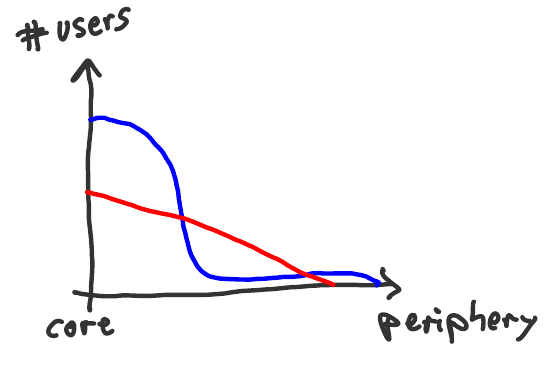
\includegraphics[width=8cm]{users-periphery.png}
}
\subsection{Release, Commits, Issue closures}
\textbf{Contributing actions}
\begin{align}
 C = \text{PushEvents} + \text{PullRequests} + c_{\text{Issues}} \text{Issues}
\end{align}

\begin{align}
 \text{Issue closing} = \frac{}{}
\end{align}


\textbf{Issue User Effectiveness:} 
\begin{align}
 IUE = \frac{\Delta \frac{\text{\# Issues Open }}{\text{\# Total Issues}}}{\Delta\text{\# User contributing}}
\end{align}



\subsection{Downloads, Forks, Views etc.}
\textbf{User activity:}
\begin{align}
 \text{UA} = c_{\text{Forks}}\text{Forks} + c_{\text{WatchEvents}} \text{WatchEvents} + c_{\text{IssueEvents}} \text{IssueEvents}
\end{align}




\section{Reference}
\subsection{Assignee from API}
Example URL: \texttt{https://api.github.com/repos/thgersdorf/github-play/issues/1}

\begin{lstlisting}
 {
  "url": "https://api.github.com/repos/kevans91/Chatters/issues/5",
  "labels_url": "https://api.github.com/repos/kevans91/Chatters/issues/5/labels{/name}",
  "comments_url": "https://api.github.com/repos/kevans91/Chatters/issues/5/comments",
  "events_url": "https://api.github.com/repos/kevans91/Chatters/issues/5/events",
  "html_url": "https://github.com/kevans91/Chatters/issues/5",
  "id": 4059710,
  "number": 5,
  "title": "Locked Menu Entries",
  "user": {
    "login": "kevans91",
    "id": 646318,
    "avatar_url": "https://gravatar.com/avatar/8d4c2928fe43bb196970867f59ab6b93?d=https%3A%2F%2Fidenticons.github.com%2F5b22ea77797a2c6e6e0859b128be4d94.png&r=x",
    "gravatar_id": "8d4c2928fe43bb196970867f59ab6b93",
    "url": "https://api.github.com/users/kevans91",
    "html_url": "https://github.com/kevans91",
    "followers_url": "https://api.github.com/users/kevans91/followers",
    "following_url": "https://api.github.com/users/kevans91/following{/other_user}",
    "gists_url": "https://api.github.com/users/kevans91/gists{/gist_id}",
    "starred_url": "https://api.github.com/users/kevans91/starred{/owner}{/repo}",
    "subscriptions_url": "https://api.github.com/users/kevans91/subscriptions",
    "organizations_url": "https://api.github.com/users/kevans91/orgs",
    "repos_url": "https://api.github.com/users/kevans91/repos",
    "events_url": "https://api.github.com/users/kevans91/events{/privacy}",
    "received_events_url": "https://api.github.com/users/kevans91/received_events",
    "type": "User",
    "site_admin": false
  },
  "labels": [
    {
      "url": "https://api.github.com/repos/kevans91/Chatters/labels/enhancement",
      "name": "enhancement",
      "color": "84b6eb"
    }
  ],
  "state": "open",
  "assignee": null,
  "milestone": null,
  "comments": 0,
  "created_at": "2012-04-11T06:43:08Z",
  "updated_at": "2012-04-11T06:43:08Z",
  "closed_at": null,
  "pull_request": {
    "html_url": null,
    "diff_url": null,
    "patch_url": null
  },
  "body": "Locked menu entries currently clutter up the menus at the top pretty badly. They either need to be removed or used.",
  "closed_by": null
}
\end{lstlisting}

\subsection{Raw JSONs}
\subsubsection{IssuesEvent}

\begin{lstlisting}
 "repository":{"homepage":"http://tdurand.github.com/mapafortaleza",
"has_downloads":true,"has_issues":true,"master_branch":"gh-pages","forks":5,"language":"JavaScript","fork":false,"has_wiki":true,"url":"https://github.com/tdurand/mapafortaleza","created_at":"2011/09/29 03:27:42 -0700","size":132,"private":false,"name":"mapafortaleza","description":"Mapa de Fortaleza","owner":"tdurand","open_issues":9,"watchers":13,"pushed_at":"2012/02/29 16:43:30 -0800"},
"actor_attributes":{"name":"Thibault Durand","company":"@tibbb","gravatar_id":"cedb88f236afaeed4caea39917ebd0a7","blog":"http://www.thibault-durand.fr","type":"User","login":"tdurand"}
,"created_at":"2012/04/11 16:01:27 -0700","public":true,"actor":"tdurand","payload":{"number":12,"action":"opened","issue":4075341},"url":"https://github.com/tdurand/mapafortaleza/issues/12","type":"
IssuesEvent"}
\end{lstlisting}

\subsubsection{CreateEvent}

\begin{lstlisting}
{"repository":{"homepage":"http://www.omegahat.org/CodeDepends","has_downloads":true,"has_issues":true,"forks":1,"fork":false,"has_wiki":true,"url":"https://github.com/duncantl/CodeDepends","created_at":"2012/04/11 15:17:31 -0700","size":0,"private":false,"name":"CodeDepends","description":"Analysis of R code for reproducible research and code view","owner":"duncantl","
open_issues":0,"watchers":1,"pushed_at":"2012/04/11 15:20:10 -0700"},"actor_attributes":{"name":"Duncan Temple Lang","gravatar_id":"be39cb3e7dc5b8133eba71370eeec525","location":"Bay Area","blog":"http://www.omegahat.org","type":"User","login":"duncantl"},"created_at":"2012/04/11 15:20:11 -0700","public":true,"actor":"duncantl","payload":{"master_branch":"master","description":"Analysis of R code for reproducible research and code view","ref_type":"branch","ref":"master"},"url":"https://github.com/duncantl/CodeDepends/compare/master","type":"CreateEvent"}
\end{lstlisting}


\subsubsection{PushEvent}

\begin{lstlisting}
{"repository":{"homepage":"","has_downloads":true,"has_issues":true,"
forks":1,"fork":false,"has_wiki":true,"url":"https://github.com/brunolopesjn/JConvexHull","created_at":"2012/04/10 18:37:34 -0700","size":208,"private":false,"name":"JConvexHull","description":"Programa Java Swing que resolve o problema do caixeiro viajante (TSP) utilizando o Convexo de Hull","owner":"brunolopesjn","open_issues":0,"watchers":1,"pushed_at":"2012/04/11 15:01:36 -0700"},"actor_attributes":{"name":"Bruno Lopes Alcantara Batista","gravatar_id":"854bf813e2a302dcc4a059b89c502424","blog":"kariridev.blogspot.com","type":"User","login":"brunolopesjn","email":"brunolopesjn@gmail.com"},"created_at":"2012/04/11 15:01:37 -0700","public":true,"actor":"brunolopesjn","payload":{"head":"8469f67ff919f2a776336bfe61f5ae7f40e76c72","size":1,"shas":[["8469f67ff919f2a776336bfe61f5ae7f40e76c72","brunolopesjn@gmail.com","Criado a interface grafica base, de desenho dos pontos, o desenho\ndo plano cartesiano e a ica de abertura de arquivos.","Bruno Lopes Alcantara Batista",true]],"ref":"refs/heads/master"},"
url":"https://github.com/brunolopesjn/JConvexHull/compare/ea77edbd70...8469f67ff9","type":"PushEvent"}
\end{lstlisting}


\subsubsection{GistEvent}
\begin{lstlisting}
{"actor_attributes":{"name":"Javi Loureiro","gravatar_id":"9cc006c8171d7af9f171cf5b2db15299","location":"Madrid","blog":"http://javiloureiro.com","type":"User","login":"sieyin"},"created_at":"2012/04/11 15:54:31 -0700","public":true,"actor":"sieyin","payload":{"name":"gist: 2363301","action":"update","url":"https://gist.github.com/2363301","id":2363301,"desc":"About Javi Loureiro"},"url":"https://gist.github.com/2363301","type":"GistEvent"
\end{lstlisting}



\subsubsection{IssueCommentEvent}
\begin{lstlisting}
{"repository":{"homepage":"","has_
downloads":true,"has_issues":true,"forks":1,"language":"JavaScript","fork":false,"has_wiki":true,"url":"https://github.com/sruecker/SET","created_at":"2012/03/14 15:59:17 -0700","size":118976,"private":false,"name":"SET","description":"Simulated Environment for Theatre, Phase I","owner":"sruecker","open_issues":36,"watchers":3,"pushed_at":"2012/04/11 15:35:27 -0700"},"actor_attributes":{"name":"Omar Rodriguez-Arenas","gravatar_id":"97f7a591e4a3160a24347bb83091d627","location":"Edmonton, AB","blog":"http://www.omarrodriguez.org/","type":"User","login":"lagoan"},"created_at":"2012/04/11 15:54:29 -0700","public":true,"actor":"lagoan","payload":{"issue_id":3880583,"comment_id":5081038},"url":"https://github.com/sruecker/SET/issues/52#issuecomment-5081038","type":"IssueCommentEvent"}
\end{lstlisting}

\subsubsection{CommitCommentEvent}
\begin{lstlisting}
{"repository":{"homepage":"","has_downloads":true,"has_issues":true,"forks":2,"language":"Java","fork":false,"has_wiki":true,"url":"https://github.com/mju/nextgenforreal","created_at":"2012/03/29 08:23:00 -0700","size":136,"private":false,"name":"nextgenforreal","description":"Next Gen For Real","owner":"mju","open_issues":0,"watchers":2,"pushed_at":"2012/03/30 05:12:13 -0700"},"actor_attributes":{"gravatar_id":"00c27eb39df73548f57a7e229962eefb","type":"User","login":"nadirabid"},"created_at":"2012/04/11 15:56:48 -0700","public":true,"actor":"nadirabid","payload":{"commit":"4390c06468a07594b7a08595be501ee56e737f1b","comment_id":1199860},"url":"
https://github.com/mju/nextgenforreal/commit/4390c06468a07594b7a08595be501ee56e737f1b#war/SecLookup/lookup.html-P5","type":"CommitCommentEvent"}
\end{lstlisting}

\subsubsection{ForkEvent}
\begin{lstlisting}
{"actor_attributes":{"name":"Kevin","type":"User","gravatar_id":"fa71428356c78bcb7c32a01fa353657f","login":"kmet31"},"created_at":"2012/04/11 15:57:57 -0700","actor":"kmet31","public":true,"type":"ForkEvent","repository":{"has_wiki":true,"language":"JavaScript","owner":"justinpincar","open_issues":0,"url":"https://github.com/justinpincar/monocle","watchers":2,"pushed_at":"2012/04/07 21:48:09 -0700","description":"","fork":false,"size":636,"has_downloads":true,"name":"monocle","has_issues":true,"homepage":"","forks":2,"private":false,"created_at":"2012/04/06 15:29:30 -0700"},"url":"https://github.com/kmet31/monocle","payload":{}}
\end{lstlisting}

\subsubsection{PullRequestEvent}
\begin{lstlisting}
{"repository":{"homepage":"https://github.com/mozilla-services/tokenserver","has_wiki":true,"open_issues":1,"language":"Python","watchers":6,"fork":false,"pushed_at":"2012/04/11 15:57:09 -0700","url":"https://github.com/mozilla-services/tokenserver","created_at":"2011/12/
23 07:39:35 -0800","size":216,"private":false,"organization":"mozilla-services","name":"tokenserver","description":"Token Server","owner":"mozilla-services","has_downloads":true,"has_issues":true,"forks":3},"actor_attributes":{"name":"Ryan Kelly","company":"Mozilla","gravatar_id":"7ad57e27678b3a70d05e9c3fb1af123e","location":"Melbourne, Australia","blog":"http://www.rfk.id.au/","type":"User","login":"rfk","email":"ryan@rfk.id.au"},"created_at":"2012/04/11 15:58:49 -0700","public":true,"actor":"rfk","payload":{"number":2,"pull_request":{"issue_url":"https://github.com/mozilla-services/tokenserver/issues/2","head":{"repo":{"name":"tokenserver","created_at":"2011-12-23T15:39:35Z","size":216,"has_wiki":true,"clone_url":"https://github.com/mozilla-services/tokenserver.git","watchers":6,"updated_at":"2012-04-11T22:57:10Z","private":false,"url":"https://api.github.com/repos/mozilla-services/tokenserver","ssh_url":"git@github.com:mozilla-services/tokenserver.git","fork":false,"git_url":"git://github.com/mozilla-
services/tokenserver.git","language":"Python","id":3040874,"pushed_at":"2012-04-11T22:57:09Z","svn_url":"https://github.com/mozilla-services/tokenserver","mirror_url":null,"open_issues":1,"has_downloads":true,"has_issues":true,"homepage":"https://github.com/mozilla-services/tokenserver","description":"Token Server","forks":3,"html_url":"https://github.com/mozilla-services/tokenserver","owner":{"gravatar_id":"a41a81f9188770933a4b54382c29cae4","avatar_url":"https://secure.gravatar.com/avatar/a41a81f9188770933a4b54382c29cae4?d=https://a248.e.akamai.net/assets.github.com%2Fimages%2Fgravatars%2Fgravatar-orgs.png","url":"https://api.github.com/users/mozilla-services","id":1066228,"login":"mozilla-services"}},"label":"mozilla-services:rfk/ttl-dict-fix","sha":"53e767319cda6b2569c362273eb12b2377944add","ref":"rfk/ttl-dict-fix","user":{"gravatar_id":"a41a81f9188770933a4b54382c29cae4","avatar_url":"https://secure.gravatar.com/avatar/a41a81f9188770933a4b54382c29cae4?d=https://a248.e.akamai.net/assets.github.com%2Fimages%
2Fgravatars%2Fgravatar-orgs.png","url":"https://api.github.com/users/mozilla-services","id":1066228,"login":"mozilla-services"}},"number":2,"created_at":"2012-04-11T22:58:48Z","merged":false,"changed_files":1,"merged_by":null,"body":"","title":"Make TTLedDict.__contains__ return False for expired items.","comments":0,"diff_url":"https://github.com/mozilla-services/tokenserver/pull/2.diff","updated_at":"2012-04-11T22:58:48Z","additions":8,"url":"https://api.github.com/repos/mozilla-services/tokenserver/pulls/2","_links":{"html":{"href":"https://github.com/mozilla-services/tokenserver/pull/2"},"self":{"href":"https://api.github.com/repos/mozilla-services/tokenserver/pulls/2"},"comments":{"href":"https://api.github.com/repos/mozilla-services/tokenserver/issues/2/comments"},"review_comments":{"href":"https://api.github.com/repos/mozilla-services/tokenserver/pulls/2/comments"}},"id":1147626,"patch_url":"https://github.com/mozilla-services/tokenserver/pull/2.patch","mergeable":null,"closed_at":null,"commits":1,"
merged_at":null,"review_comments":0,"html_url":"https://github.com/mozilla-services/tokenserver/pull/2","user":{"gravatar_id":"7ad57e27678b3a70d05e9c3fb1af123e","avatar_url":"https://secure.gravatar.com/avatar/7ad57e27678b3a70d05e9c3fb1af123e?d=https://a248.e.akamai.net/assets.github.com%2Fimages%2Fgravatars%2Fgravatar-140.png","url":"https://api.github.com/users/rfk","id":34695,"login":"rfk"},"deletions":0,"base":{"repo":{"name":"tokenserver","created_at":"2011-12-23T15:39:35Z","size":216,"has_wiki":true,"clone_url":"https://github.com/mozilla-services/tokenserver.git","watchers":6,"updated_at":"2012-04-11T22:57:10Z","private":false,"url":"https://api.github.com/repos/mozilla-services/tokenserver","ssh_url":"git@github.com:mozilla-services/tokenserver.git","fork":false,"git_url":"git://github.com/mozilla-services/tokenserver.git","language":"Python","id":3040874,"pushed_at":"2012-04-11T22:57:09Z","svn_url":"https://github.com/mozilla-services/tokenserver","mirror_url":null,"open_issues":1,"has_downloads":
true,"has_issues":true,"homepage":"https://github.com/mozilla-services/tokenserver","description":"Token Server","forks":3,"html_url":"https://github.com/mozilla-services/tokenserver","owner":{"gravatar_id":"a41a81f9188770933a4b54382c29cae4","avatar_url":"https://secure.gravatar.com/avatar/a41a81f9188770933a4b54382c29cae4?d=https://a248.e.akamai.net/assets.github.com%2Fimages%2Fgravatars%2Fgravatar-orgs.png","url":"https://api.github.com/users/mozilla-services","id":1066228,"login":"mozilla-services"}},"label":"mozilla-services:master","sha":"2ef48e3d3e57030597175149703a362ed9794335","ref":"master","user":{"gravatar_id":"a41a81f9188770933a4b54382c29cae4","avatar_url":"https://secure.gravatar.com/avatar/a41a81f9188770933a4b54382c29cae4?d=https://a248.e.akamai.net/assets.github.com%2Fimages%2Fgravatars%2Fgravatar-orgs.png","url":"https://api.github.com/users/mozilla-services","id":1066228,"login":"mozilla-services"}},"state":"open"},"action":"opened"},"url":"https://github.com/mozilla-services/tokenserver/pull/
2","type":"PullRequestEvent"
\end{lstlisting}


\subsubsection{PullRequestReviewCommentEvent}
\begin{lstlisting}
{"repository":{"homepage":"","has_downloads":true,"has_issues":true,"
forks":6,"language":"Python","fork":false,"has_wiki":true,"organization":"pinax","url":"https://github.com/pinax/django-user-accounts","created_at":"2012/03/10 13:41:14 -0800","size":172,"private":false,"name":"django-user-accounts","description":"User accounts for Django","owner":"pinax","open_issues":2,"watchers":13,"pushed_at":"2012/04/11 15:34:45 -0700"},"actor_attributes":{"name":"Brian Rosner","company":"Eldarion, Inc.","gravatar_id":"b7472bc7aa45c70641c299e9408b78ab","location":"Denver, CO","blog":"http://brosner.com/","type":"User","login":"brosner","email":"brosner@gmail.com"},"created_at":"2012/04/11 15:59:05 -0700","public":true,"actor":"brosner","payload":{"comment":{"position":13,"created_at":"2012-04-11T22:59:05Z","original_commit_id":"9fcdbf959760964592fb8537551cd1a95eed5a58","body":"The code you have in ``conf.py`` is correct. This line is incorrect because ``appconf`` prefixes what you add in the conf with ``ACCOUNT``.","original_position":13,"commit_id":"
9fcdbf959760964592fb8537551cd1a95eed5a58","updated_at":"2012-04-11T22:59:05Z","url":"https://api.github.com/repos/pinax/django-user-accounts/pulls/comments/673911","id":673911,"path":"account/fields.py","user":{"gravatar_id":"b7472bc7aa45c70641c299e9408b78ab","avatar_url":"https://secure.gravatar.com/avatar/b7472bc7aa45c70641c299e9408b78ab?d=https://a248.e.akamai.net/assets.github.com%2Fimages%2Fgravatars%2Fgravatar-140.png","url":"https://api.github.com/users/brosner","id":124,"login":"brosner"}}},"url":"https://github.com/pinax/django-user-accounts/pull/11#discussion-diff-673911","type":"PullRequestReviewCommentEvent"
\end{lstlisting}


\subsubsection{WatchEvent}
\begin{lstlisting}
{"repository":{"homepage":"www.meteor.com","has_downloads":true,"has_issues":true,"forks":54,"language":"JavaScript","fork":false,"has_wiki":true,"organization":"meteor","url":"https://github.com/meteor/meteor","
created_at":"2012/01/18 17:58:17 -0800","size":292,"private":false,"name":"meteor","description":"Meteor, an ultra-simple, database-everywhere, data-on-the-wire, pure-Javascript web framework.","owner":"meteor","open_issues":18,"watchers":1322,"pushed_at":"2012/04/11 14:20:18 -0700"},"actor_attributes":{"name":"Christian Giordano","gravatar_id":"c36cef01195c0a581ece67aa81ee40a8","location":"London","blog":"http://nuthinking.com","type":"User","login":"nuthinking","email":"christian@nuthinking.com"},"created_at":"2012/04/11 15:58:11 -0700","public":true,"actor":"nuthinking","payload":{"action":"started"},"url":"https://github.com/meteor/meteor","type":"WatchEvent"
\end{lstlisting}

\subsubsection{FollowEvent}
\begin{lstlisting}
{"actor_attributes":{"name":"David A. Dalrymple","company":"MIT","gravatar_id":"d6a774b6c841325abf20e8c2b1cfb43b","location":"Cambridge, MA","blog":"http://davidad.net","type":"User","login":"davidad","email":"davidad@alum.mit.edu"},"created_at":"2012/04/11 15:58:41 -0700","public":true,"actor":"davidad","payload":{"target":{"gravatar_id":"237338834f2f8948e862e91392a8c1b4","followers":9,"id":40273,"repos":17,"login":"saizai"}},"url":"https://github.com/saizai","type":"FollowEvent"}
\end{lstlisting}


\subsubsection{GollumEvent}
\begin{lstlisting}
{"repository":{"homepage":"http://www.sisodb.com","has_downloads":true,"has_issues":true,"forks":4,"language":"C#","fork":false,"has_wiki":true,"url":"https://github.com/
danielwertheim/SisoDb-Provider","created_at":"2011/01/31 05:33:16 -0800","size":3472,"private":false,"name":"SisoDb-Provider","description":"SisoDb - Simple Structure Oriented Db","owner":"danielwertheim","open_issues":0,"watchers":52,"pushed_at":"2012/04/11 14:52:42 -0700"},"actor_attributes":{"name":"Daniel Wertheim","gravatar_id":"274ce0291206c9d27635a865ac48b5c4","location":"Sweden","blog":"http://daniel.wertheim.se","type":"User","login":"danielwertheim"},"created_at":"2012/04/11 15:01:37 -0700","public":true,"actor":"danielwertheim","payload":{"pages":[{"sha":"909e1049863468ad462655505441bf7bf39dc739","title":"Release notes","action":"edited","page_name":"Release notes","summary":null,"html_url":"https://github.com/danielwertheim/SisoDb-Provider/wiki/Release-notes"}]},"url":"https://github.com/danielwertheim/SisoDb-Provider/wiki/Release-notes","type":"GollumEvent"}
\end{lstlisting}

\subsubsection{DeleteEvent}
\begin{lstlisting}
{"repository":{"homepage":"","has_downloads":true,"has_issues":false,"master_branch":"master","forks":0,"language":"Shell","fork":true,"has_wiki":true,"url":"https://github.com/travp624/android_device_moto_shadow","created_at":"2012/04/03 01:32:24 -0700","size":6060,"private":false,"name":"android_device_moto_shadow","description":"","owner":"travp624","open_issues":0,"watchers":1,"pushed_at":"2012/04/11 15:02:07 -0700"},"actor_attributes":{"name":"teamicemods","gravatar_id":"1eb4d77c7c79eccde05a7047fbae4195","location":"wisconsin home of cheese baby","blog":"","type":"User","login":"travp624","email":"travp624@gmail.com"},"created_at":"2012/04/11 15:02:07 -0700","public":true,"actor":"travp624","payload":{"ref_type":"branch","ref":"ics"},"url":"https://github.com/","type":"DeleteEvent"}
\end{lstlisting}






\subsubsection{MemberEvent}
\begin{lstlisting}
{"repository":{"homepage":"","has_downloads":true,"has_issues":true,"forks":1,"language":"Python","fork":false,"has_wiki":true,"url":"https://github.com/olleicua/Py4colorReduction","created_at":"2012/04/11 12:58:45 -0700","size":92,"private":false,"name":"Py4colorReduction","description":"A project to reduce graph configurations as part of the four color theorem proof in Python","owner":"olleicua","open_issues":0,"watchers":1,"pushed_at":"2012/04/11 15:14:51 -0700"},"actor_attributes":{"gravatar_id":"a6b8d1d40e9a7f8689c796755412638d","type":"User","login":"olleicua"},"created_at":"2012/04/11 15:54:06 -0700","public":true,"actor":"olleicua","payload":{"member":{"avatar_url":"https://secure.gravatar.com/avatar/
8a5e72675540095c6ca3d7825d2c2451?d=https://a248.e.akamai.net/assets.github.com%2Fimages%2Fgravatars%2Fgravatar-140.png","gravatar_id":"8a5e72675540095c6ca3d7825d2c2451","url":"https://api.github.com/users/emzeidan","id":1634836,"login":"emzeidan"},"action":"added"},"url":"https://github.com/olleicua/Py4colorReduction","type":"MemberEvent"}
\end{lstlisting}

\subsubsection{DownloadEvent}
\begin{lstlisting}
{"repository":{"homepage":"","has_downloads":true,"has_issues":true,"forks":0,"language":"Java","fork":true,"has_wiki":false,"organization":"disy","url":"https://github.com/disy/jax-rx","created_at":"2011/09/13 06:02:16 -0700","size":212,"private":false,"name":"jax-rx","description":"JAX-RX (REST) Interface, REST on XML easy made","owner":"disy","open_issues":0,"watchers":2,"pushed_at":"2012/04/06 23:31:00 -0700"},"actor_attributes":{"name":"Sebastian Graf","company":"University of Konstanz","gravatar_id":"0409cd1da7452f896e86b7a6ebd9b85a","location":"Konstanz, Germany","blog":"http://www.informatik.uni-konstanz.de/arbeitsgruppen/disy/members/sebastian-graf/","type":"User","login":"sebastiangraf","email":"sebastian.graf@uni-konstanz.de"},"
created_at":"2012/04/11 15:52:20 -0700","public":true,"actor":"sebastiangraf","payload":{"url":"https://github.com/downloads/disy/jax-rx/jax-rx-1.3.3-SNAPSHOT.jar","id":218663},"url":"https://github.com/downloads/disy/jax-rx/jax-rx-1.3.3-SNAPSHOT.jar","type":"DownloadEvent"}
\end{lstlisting}

\subsubsection{PublicEvent}
\begin{lstlisting}
{"repository":{"homepage":"","has_downloads":true,"has_issues":true,"forks":1,"language":"C++","fork":false,"has_wiki":true,"url":"https://github.com/brendonjustin/trees","created_at":"2012/04/11 15:20:22 -0700","size":124,"
private":false,"name":"trees","description":"","owner":"brendonjustin","open_issues":0,"watchers":1,"pushed_at":"2012/04/11 15:21:13 -0700"},"actor_attributes":{"name":"Brendon Justin","gravatar_id":"d0593bd249a5194e00483ac594128566","type":"User","login":"brendonjustin"},"created_at":"2012/04/11 15:22:25 -0700","public":true,"actor":"brendonjustin","url":"https://github.com/brendonjustin/trees","type":"PublicEvent"}
\end{lstlisting}













\subsection{SQL Queries Temp}
\lstset{
	backgroundcolor=\color{lbcolor},
	tabsize=4,
	rulecolor=,
	language=SQL,
	numbers=left,
	numberstyle=\footnotesize,
        basicstyle=\scriptsize,
        upquote=true,
        aboveskip={0.3\baselineskip},
        columns=fixed,
        showstringspaces=false,
        extendedchars=true,
        breaklines=true,
        prebreak = \raisebox{0ex}[0ex][0ex]{\ensuremath{\hookleftarrow}},
        frame=single,
        showtabs=false,
        showspaces=false,
        showstringspaces=false,
	basicstyle=\small\ttfamily,
        identifierstyle=\ttfamily,
%         keywordstyle=\color[rgb]{0,0,1},
        commentstyle=\color[rgb]{0.133,0.545,0.133},
        stringstyle=\color[rgb]{0.627,0.126,0.941},
}


\subsubsection{Generic Event Queries}
\begin{lstlisting}
 # total events involvements:
 SELECT * FROM `events` WHERE `actor` = 'mitar' AND `repository_owner` != 'mitar'
SELECT * FROM `events` WHERE `actor` = 'mitar' AND `repository_owner` = 'mitar'

 # specific Issues properties
 SELECT payload_number, payload_action, payload_issue from events where type   = 'IssuesEvent' LIMIT 30;


# user profiling
INSERT INTO eng_users (user, TotalEvents,  IssuesEvent , CreateEvent , PushEvent , GistEvent , IssueCommentEvent , CommitCommentEvent , ForkEvent , WatchEvent , PullRequestEvent , PullRequestReviewCommentEvent , FollowEvent , GollumEvent , DeleteEvent , MemberEvent , DownloadEvent , PublicEvent, Issues_Opened, Issues_Closed, Events_Own, Events_Active_Involvement, Events_Passive_Involvment)  SELECT '" + user_i[0] +"' , COUNT(*),  SUM(Type = 'IssuesEvent'),  SUM(Type = 'CreateEvent'), SUM(Type = 'PushEvent'), SUM(Type = 'GistEvent'), SUM(Type = 'IssueCommentEvent'),SUM(Type = 'CommitCommentEvent'),SUM(Type = 'ForkEvent'),SUM(Type = 'WatchEvent'),SUM(Type = 'PullRequestEvent'),SUM(Type = 'PullRequestReviewCommentEvent'),SUM(Type = 'FollowEvent'),SUM(Type = 'GollumEvent'),   SUM(Type = 'DeleteEvent'), SUM(Type = 'MemberEvent'), SUM(Type = 'DownloadEvent'), SUM(Type = 'PublicEvent'), SUM(type = 'IssuesEvent' AND payload_action='opened'), SUM(type = 'IssuesEvent' AND payload_action='closed'),   SUM(actor = '" + 
user_i[0] +"' AND `repository_owner` = '" + user_i[0] +"'),  SUM(actor = '" + user_i[0] +"' AND `repository_owner` != '" + user_i[0] +"') , SUM( actor != '" + user_i[0] +"' AND `repository_owner` = '" + user_i[0] +"'   )   FROM events WHERE actor_attributes_type = 'User' AND actor_attributes_login = '" + user_i[0] +"' ON DUPLICATE KEY UPDATE user = '" + user_i[0] +"' ;
# passive involvement:
UPDATE eng_users SET Events_Passive_Involvment = ( SELECT COUNT( * )  FROM  `events`  WHERE  `repository_organization` IS NULL  AND   `repository_owner` =  'torvalds' AND actor !=  'torvalds' )  WHERE eng_users.user =  'torvalds'




# user commit networking:
SELECT *  FROM  `events`  WHERE  `type` LIKE  'PullRequestEvent' AND  `payload_action` LIKE  'Closed' AND  `repository_url` LIKE  'https://github.com/rails/rails'
SELECT DISTINCT(CONCAT(actor,payload_pull_request_head_repo_owner_login)),actor,payload_pull_request_head_repo_owner_login
FROM  `events`  WHERE  `type` LIKE  'PullRequestEvent' AND  `payload_action` LIKE  'Closed' AND  `repository_url` LIKE  'https://github.com/rails/rails'
\end{lstlisting}


\section{SQL Database Performance Optimization}
Lessons learned:
\begin{itemize}
 \item 
\end{itemize}



\end{document}

